\documentclass[handout]{beamer}
\usepackage{verbatim}
\usepackage{xcolor}
\usepackage{multirow}
\usepackage{amssymb}
\usepackage{tikz}
\usepackage{hyperref}
\usetikzlibrary{positioning,fit}
%\usepackage{enumitem}
\usetheme{Warsaw}
\setbeamertemplate{navigation symbols}{}
\newcommand{\blue}[1]{{\color{blue} #1}}
\newcommand{\red}[1]{{\color{red} #1}}
\newcommand{\grn}[1]{{\color{green} #1}}
\newcommand{\bluRed}[2]{{\color{blue} #1}{\color{red} #2}}
\newcommand{\qtns}[0]{\begin{center} Questions? \end{center}}
\newcommand{\nl}[1]{\vspace{#1 em}}
\newcommand{\cntrImg}[2]{\begin{center}\includegraphics[scale=#2]{#1}\end{center}}
\newcommand{\defn}[1]{{\bf #1}}
\let\emptyset\varnothing
\newcommand{\SampS}[0]{$\mathcal{S}$}

\title{Math 3070, Applied Statistics}

\begin{document}

\begin{frame}
    \begin{beamercolorbox}[rounded=true,wd=\textwidth,center]{title}
        \usebeamerfont{title}\inserttitle
    \end{beamercolorbox}
    \begin{center}
        Section 1\\
        \nl{0.5}
        September 25, 2019
    \end{center}
\end{frame}
\begin{frame}{Lecture Outline, 9/25}
    Section 4.3
    \begin{itemize}
        \item Normal Random Variables
        \item Mean and Variance of the Standard Normal
        \item Z-Transform
        \item CDF of a Standard Normal
        \item Examples
    \end{itemize}
\end{frame}
\begin{frame}{Normal Random Variables, PDF}
    \begin{block}{}
        A random variable $X$ follows a \textbf{normal distribution} with mean $\mu$ and standard deivation $\sigma$ if has the following PDF.
        $$ f(x) = \frac{1}{\sqrt{2\pi} \sigma} \exp\bigg(\frac{-(x-\mu)^2}{2\sigma^2}\bigg) $$
        $X\sim N(\mu,\sigma)$
    \end{block}
    \begin{block}{}
        The $N(0,1)$ distribution is the \textbf{standard normal distribution}.
    \end{block}
    \begin{center}
        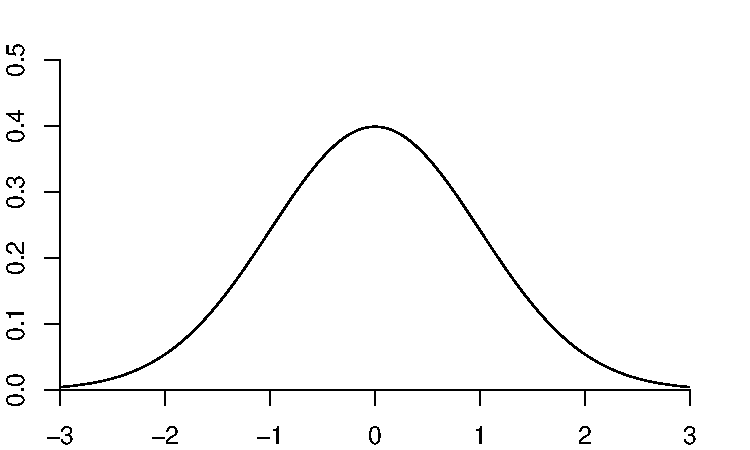
\includegraphics[scale=.4]{ch4_pdf_norm.pdf}
    \end{center}
    \vfill
\end{frame}
\begin{frame}{Normal Random Variables, Importance}
    Normal distributions often sufficiently model large sample (large $n$) statistics via Central Limit Theorem. \\ \nl{0.5}
    In this course, it will be used extensively when applying the central limit theorem.
\end{frame}

\begin{frame}{Standard Normal Distribution, Integral of PDF}
    We want to show that the standard normal pdf is a valid pdf. \\
    Have that $f(x)\geq 0$. Need to show $\int_{-\infty}^\infty f(x) dx = 1$.

    \vspace{.2cm}
    We will use the special integral $\int_{-\infty}^\infty e^{-x^2}\ dx=\sqrt\pi$.
    \url{https://en.wikipedia.org/wiki/Gaussian_integral}
    \\
    \pause \vspace{.2cm}
    Assuming this, substituting $u=x/\sqrt2$,
    \begin{align*}
        \uncover<4->{\int_{-\infty}^\infty \phi(x)\ dx & = \frac1{\sqrt{2\pi}}\int_{-\infty}^\infty e^{-x^2/2}\ dx \\}
        \uncover<5->{                                  & = \frac1{\sqrt{\pi}}\int_{-\infty}^\infty e^{-u^2}\ du \\}
        \uncover<6->{                                  & = \frac1{\sqrt{\pi}}\cdot\sqrt{\pi} = 1}
    \end{align*}

\end{frame}

\begin{frame}{Mean of Standard Normal}
    The standard normal distribution is symmetric in the sense that the pdf $\phi(x)$ is an even function, i.e., $\phi(-x)=\phi(x)$:
    $$\phi(x)=\frac1{\sqrt{2\pi}}e^{-x^2/2}$$
    \pause Therefore the mean of a standard normal random variable is
    $$E(X)=\int_{-\infty}^\infty x\phi(x)\ dx =\int_{-\infty}^\infty x\cdot\frac1{\sqrt{2\pi}}e^{-x^2/2}\ dx=0$$
    since the integrand is an odd function.
    \begin{center}
        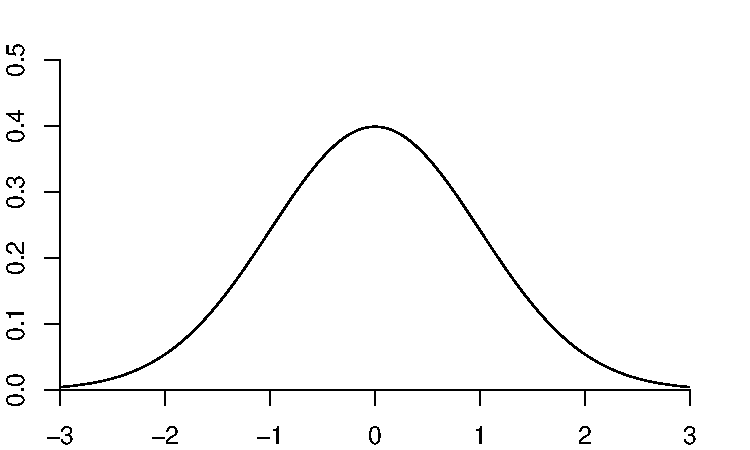
\includegraphics[scale=.5]{ch4_pdf_norm.pdf}
    \end{center}
\end{frame}
\begin{frame}{Variance of Standard Normal}
    Substituting $u=x^2/2$, note that
    \begin{align*}
        \int xe^{-x^2/2}\ dx = \int e^{-u}\ du = -e^{-u} = -e^{-x^2/2}
    \end{align*}

    \pause Integrating by parts,
    \begin{align*}
        V(X)          & =E[(X-\mu)^2] = E(X^2) = \int_{-\infty}^\infty x^2f(x)\ dx                                                                                   \\
        \uncover<3->{ & = \frac1{\sqrt{2\pi}}\int_{-\infty}^\infty x\cdot xe^{-x^2/2}\ dx \\}
        \uncover<4->{ & = \frac1{\sqrt{2\pi}}\left[x(-e^{-x^2/2})\big\vert_{-\infty}^\infty + \int_{-\infty}^\infty e^{-x^2/2}\ dx \right] \\}
        \uncover<5->{ & = \frac1{\sqrt{2\pi}}\int_{-\infty}^\infty e^{-x^2/2}\ dx=1}
    \end{align*}
    \uncover<6->{\vspace{-.35cm}
        \begin{block}{}
            A standard normal random variable has mean 0 and variance 1.
        \end{block}}
\end{frame}
\begin{frame}{Z-Transform, Motivation}
    By now, we can see that normal distributions are non-trivial to integrate. Luckily, probabilities can still be computed using Z-transforms.
    \begin{block}{}
        Given $Z \sim N(0,1)$ or $Z$ is a standard normal,
        $$\sigma Z + \mu  \sim N(\mu,\sigma).$$
        The equivalently or more commonly used fact is the \textbf{Z-Transform}:
        $$ X\sim N(\mu,\sigma) \to \frac{X-\mu}{\sigma} \sim N(0,1) $$
    \end{block}
    Use the Z-Transform to change integrals or probabilities involving and normal random variable into ones involving the standard normal. The later can be looked up in tables such as Table A3.
\end{frame}
\begin{frame}{Z-Transform, Proof and Calculation}
    Let $X \sim N(\mu,\sigma)$ and $Z\sim N(0,1)$. If the PDF of $X$ and $\sigma Z + \mu$ match, then they follow the same distribution.\\ \nl{0.5}
    Start with the CDF of $\sigma Z + \mu$.
\begin{align*} 
    P(\sigma Z + \mu < x)  & = P\bigg(Z < \frac{x-\mu}{\sigma}\bigg) \\
    &= \int_{-\infty}^{\frac{x-\mu}{\sigma}} \frac{1}{\sqrt{2 \pi}} \exp \bigg( \frac{-y^2}{2}\bigg) dy\\
\end{align*}
\pause Differentiate to show that the PDFs are the same.
\pause \begin{align*} 
    \frac{d}{dx}P(\sigma Z + \mu < x)  & = \frac{d}{dx}\int_{-\infty}^{\frac{x-\mu}{\sigma}} \frac{1}{\sqrt{2 \pi}} \exp \bigg( \frac{-y^2}{2}\bigg) dy\\
    & = \frac{1}{\sqrt{2 \pi}} \exp \bigg( \frac{-(x-u)^2}{2\sigma^2}\bigg) \frac{1}{\sigma}
\end{align*}
Note: Fundamental Theorem of Calculus and Chain Rule used.
\end{frame}
\begin{frame}{Z-Transform, Proof and Calculation}
    The derivative of the CDF of $\sigma Z + \mu$ and PDF of $X$ are equal meaning that they behave the exact same way as random variables. They not the same variable, but have their events have the same probabilities.
    $$ P(X<x) = P\bigg(\frac{X-\mu}{\sigma}< \frac{x-\mu}{\sigma}\bigg) = P\bigg(Z< \frac{x-\mu}{\sigma}\bigg)$$
    \pause Moreover, this gives us a way to directly compute probabilities many events involving any random variable in terms of standard random variables.
    \nl{0.5}
    Notice that the left hand side is difficult if not impossible to integrate while the right hand side can be looked up as long as all non-random variables are known.
\end{frame}
\begin{frame}{Z-Transform, Mean and Variance of Normal Distributions}
    Since $X$ and $\sigma Z + \mu$ have the same PDF.
    $$ E[X] = E[\sigma Z + \mu] = \sigma E[Z] + \mu = \mu $$
    $$ V(X) = V(\sigma Z + \mu) = \sigma^2 V(Z) =\sigma^2 $$
    $$ \text{standard deviation of } X = \sigma  $$
    \vfill
\end{frame}
\begin{frame}{CDF of a Standard Normal}
    \begin{block}{}
        The CDF of the a standard normal random variable $N(0,1)$ is denoted below. It is denoted since it frequently appears in calculations involving normal random variables.
        $$\Phi(x) = \frac{1}{\sqrt{2\pi}}\int_{-\infty}^x \exp \bigg(\frac{-y^2}{2}\bigg) dy$$
    \end{block}
    Values of $\Phi(x)$ can be looked up by using Table A.3. Your calculator should have the ability to look up values as well.
    \vfill
\end{frame}
\begin{frame}{CDF of a Standard Normal, Critical Values}
    \begin{block}{}
        The critical value $z_\alpha$ is defined as
        $$ \alpha = 1 - \Phi(z_\alpha) = P(Z\geq z_\alpha)$$
        and is equal to the $100(1-\alpha)^{th}$ percentile.
        \\
        Due to symmetry of the standard normal,
        $$ \alpha = \Phi(-z_\alpha) = P(Z\leq -z_\alpha)$$
    \end{block}
    $68-95-99.7$ Rule:
    \begin{itemize}
        \item $P(-1<Z<1)=P(-\sigma <X-\mu < \sigma)\approx 68\%$
        \item $P(-2<Z<2)=P(-2\sigma <X-\mu < 2\sigma)\approx 95\%$
        \item $P(-3<Z<3)=P(-3\sigma <X-\mu < 3\sigma)\approx 99.7\%$
    \end{itemize}
    \vfill
\end{frame}
\begin{frame}{Simple Example, Using Z-Transforms}
    The weight of an Altoid $X$ follows a normal distribution with a mean of 16 grams and standard deviation of 1.2 grams. What is the probability that a randomly selected Altoid less than 17 grams in weight?
    \\ \nl{0.5}
    \begin{align*}
        P(X<17) & \uncover<1->{= P\bigg(\frac{X-16}{1.2}< \frac{17-16}{1.2}\bigg)}\\
        & \uncover<2->{ = \Phi\bigg(\frac{17-16}{1.2}\bigg)} \\
        & \uncover<3->{ \approx 0.7967} \\
    \end{align*}
    \vfill
\end{frame}
\begin{frame}{Example, Using Z-Transforms with Absolute Values}
    The weight of an Altoid $X$ follows a normal distribution with a mean of 16 grams and standard deviation of 1.2 grams. What is the probability that a randomly selected Altoid is no more than 0.5 grams away from 17 grams in weight?
    \\ \nl{0.5}
    \begin{align*}
        P(|X-17|<0.5) & \uncover<1->{= P(-0.5<X-17<0.5)}\\
        & \uncover<2->{ = P(16.5<X<17.5)} \\
        & \uncover<3->{ = P\bigg(\frac{16.5-16}{1.2}<\frac{X-16}{1.2}<\frac{17.5-16}{1.2}\bigg)} \\
        & \uncover<4->{ = P\bigg(\frac{16.5-16}{1.2}<Z<\frac{17.5-16}{1.2}\bigg)} \\
        & \uncover<5->{ = \Phi \bigg(\frac{17.5-16}{1.2}\bigg) - \Phi\bigg(\frac{16.5-16}{1.2}\bigg)} \\
        & \uncover<6->{\approx 0.8944 - 0.6628 = 0.2316 } \\
    \end{align*}
\end{frame}
\begin{frame}{Example, Percentiles}
    The weight of an Altoid $X$ follows a normal distribution with a mean of 16 grams and standard deviation of 1.2 grams. Under what weight are 75\% of Altoids?
    \\ \nl{0.5}
    \pause Find $z_{75}$
    \pause $$ P(0.68) \approx 0.75 \to z_{75} \approx 0.68 $$
    \pause Use Z-Transform.
    \begin{align*}
        0.75 \approx P(Z<0.68) & \uncover<1->{= P(1.2Z+16<1.2\cdot 0.68 +16)}\\
        & \uncover<2->{ = P(X<16.816)} \\
    \end{align*}
    \pause Roughly 75\% of Altoids are under 16.816 grams.
\end{frame}
\begin{frame}{Example, Percentiles with Absolute Values}
    $X$ follows a normal distribution with a mean of 4 and standard deviation of 0.4. Determine $c$ so that 
    $$P(c \leq |X-4|)=0.5.$$
    \begin{align*}
        0.5 = P(c \leq |X-4|) & \uncover<1->{= 1 - P(|X-4|<c)}  \uncover<2->{ = 1 -P(-c < X-4 < c)} \\
        & \uncover<3->{ = 1 -P\bigg(-\frac{c}{0.4} < \frac{X-4}{0.4} < \frac{c}{0.4}\bigg)} \\
        & \uncover<4->{ = 1 -P\bigg(-\frac{c}{0.4} < Z < \frac{c}{0.4}\bigg)} \\
        & \uncover<5->{ = 1 -\bigg[\Phi\bigg(\frac{c}{0.4}\bigg) - \Phi\bigg(-\frac{c}{0.4}\bigg)\bigg]} \\
        & \uncover<6->{ = 1 -\bigg[\Phi\bigg(\frac{c}{0.4}\bigg) - \bigg(1 - \Phi\bigg(\frac{c}{0.4}\bigg)\bigg)\bigg]} \\
        & \uncover<7->{ = 2 - 2 \Phi\bigg( \frac{c}{0.4} \bigg)} \\
    \end{align*}
\end{frame}
\begin{frame}{Example, Percentiles with Absolute Values}
    $X$ follows a normal distribution with a mean of 4 and standard deviation of 0.4. Determine $c$ so that 
    $$P(c \leq |X-4|)=0.5.$$    
    $$0.25 = 1 -  \Phi\bigg( \frac{c}{0.4} \bigg) \to \uncover<1->{\Phi\bigg( \frac{c}{0.4} \bigg) =0.75}$$
    \uncover<2-> {Find the critical value, $z_{75}\approx 0.68$}
    $$ \uncover<3->{\frac{c}{0.4} \approx 0.68 \to c \approx 0.272 }$$
\end{frame}
\begin{frame}{Summary}
    \begin{itemize}
        \item $X\sim N(\mu,\sigma)$ means $X$ is normal distributed with mean $\mu$ and standard deviation $\sigma$. Its PDF is
        $$ f(x) = \frac{1}{\sigma\sqrt{2\pi}} \exp\bigg( \frac{-(x-\mu)^2}{2 \sigma^2} \bigg) $$
        \item $X\sim N(0,1)$ is a standard normal random variable.
        \item Z-Transform
        $$ \frac{X-\mu}{\sigma} \sim N(0,1) \hskip 2em \sigma Z + \mu \sim N(\mu,\sigma) $$
        \item CDF of $Z$ is denoted as $\Phi(x)$, useful in calculations.
        \item $\alpha = 1 - \Phi(z_{\alpha})$ and  $\alpha = \Phi(-z_{\alpha})$, the distribution is symmetric.
        \item $68-95-99.7$ Rule
        \item For any random variable, $P(|X|<c) = P(-c < X < c)$.
    \end{itemize}
\end{frame}
\end{document}